\section{Osmé cvičení}

\subsection{Příklad}    \noindent
K automatu $M$, který je dán následující tabulkou, zkostruujte regulární gramatiku $\mathcal{G}$, která generuje jazyk 
$L = L(M)$. 

$M$: \hspace{2mm}
\begin{minipage}{0.4\textwidth}    
    \begin{tabular}{|r c|c c|} 
        \hline
         & & $a$ & $b$ \\
        \hline
        \hline
        $\leftrightarrow$&$ A$ & $A,C$ & $B$ \\
        \hline
        &$ B$ & $\emptyset$ & $B, D$ \\
        \hline
        $\leftarrow$ &$ C$ & $\emptyset$ & $\emptyset$ \\
        \hline
        $\rightarrow$&$D$ & $A$ & $C,D$ \\
        \hline
    \end{tabular}

    \vspace*{5mm}
    $\mathcal{G} = (N, \Sigma, S, P)$ \\
    $ N = \{S, A, B, C, D\}$\\ 
    $\Sigma = \{a, b\}$

\end{minipage}\begin{minipage}{0.5\textwidth}
    mám více vstupů $\rightarrow$ přidám si $S$ 

\begin{tikzpicture}[shorten >=1pt,node distance=20mm,on grid,auto]
        \tikzstyle{every state}=[fill={rgb:black,1;white,10}, minimum size=18pt, inner sep=1pt]
    \node[state, initial] (S) {$S$}; 
    \node[state] (A) [right  of=S] {$A$}; 
    \node[state] (B) [below  of=A] {$B$}; 
    \node[state, accepting] (C) [right  of=A] {$C$}; 
    \node[state] (D) [below of=S] {$D$}; 
    
    \path[->]
    (S) edge [bend left] node {$\varepsilon$} (A)
    (S) edge [bend right] node {$\varepsilon$} (D)
    (A) edge [loop above] node {$a$} ()
    (A) edge [bend left] node {$a$} (C)
    (A) edge [bend left] node {$b$} (B)
    (B) edge [bend left] node {$b$} (D)
    (B) edge [loop right] node {$b$} ()
    (D) edge [loop left] node {$b$} ()
    (D) edge [left] node {$b$} (C)
    (D) edge [left] node {$a$} (A)
    ;    
\end{tikzpicture}

\[
    \hspace*{-45mm}
    \begin{array}{l l}
        P: & S \rightarrow A \mid D \\
        & A \rightarrow aA \mid aC \mid bB \mid \varepsilon\\
        & B \rightarrow bB \mid bD \\
        & C \rightarrow \varepsilon \\
        & D \rightarrow aA \mid bD \mid aA \\
    \end{array}
\]

\end{minipage}

\subsection{Příklad}
\noindent
Ke gramatice $\mathcal{G}$ typu 3 zkonstruujte konečný automat, který přijímá jazyk $L(\mathcal{G})$. Gramatika 
$\mathcal{G} = (N, \{a,b\}, S, P)$, kde $N = \{S, A, B\}$ a pravidla jsou 
\[
    \begin{array}{l l}
        P: & S \rightarrow abA \mid aB \\
        & A \rightarrow aA \mid aaA \mid a\\
        & B \rightarrow bB \mid b \\
    \end{array}
\]

\begin{minipage}{0.5\textwidth}
    
    \[
        \begin{array}{l l l}
            P: & S \rightarrow abA \mid aB & \text{překáží mi } \ii{abA}\\
            & C \rightarrow bA & \\ 
            & S \rightarrow aC \mid aB & \text{nové pravidlo \ii{S}} \\
            & A \rightarrow aA \mid aaA \mid a & \text{zase nám vadí } \ii{aaA}\\
            & D \rightarrow aA & \\
            & E \rightarrow \varepsilon & \\
            & A \rightarrow aA \mid aD \mid aE & \text{nové pravidlo \ii{A}} \\
            & B \rightarrow bB \mid bE & \text{nové pravidlo \ii{B}} \\
        \end{array}
        \]
\end{minipage}
\begin{minipage}{0.3\textwidth}
\end{minipage}
\begin{minipage}{0.5\textwidth}
    sestavím automat podle nových pravidel

    \begin{tikzpicture}[shorten >=1pt,node distance=20mm,on grid,auto]
    \tikzstyle{every state}=[fill={rgb:black,1;white,10}, minimum size=18pt, inner sep=1pt]
    \node[state, initial] (S) {$S$}; 
    \node[state] (B) [below  of=S] {$B$}; 
    \node[state] (C) [right  of=S] {$C$}; 
    \node[state] (A) [right  of=C] {$A$}; 
    \node[state] (D) [below of=A] {$D$}; 
    \node[state, accepting] (E) [below of=C] {$E$}; 
    
    \path[->]
    (S) edge [bend left] node {$a$} (C)
    (S) edge [bend right] node {$a$} (B)
    (C) edge [bend left] node {$b$} (A)
    (A) edge [loop right] node {$a$} ()
    (A) edge [bend right] node {$a$} (E)
    (A) edge [bend left] node {$a$} (D)
    (B) edge [loop below] node {$b$} ()
    (B) edge [bend right] node {$b$} (E)
    (D) edge [bend left] node {$a$} (A)
    ;    
\end{tikzpicture}
\end{minipage}

\newpage
\subsection{Příklad}\noindent
Je dán derivační strom v bezkontextové gramatice:


\begin{center}
        
    \begin{forest}
        for tree={
            grow=south,                 % Tree grows downward
            edge={->},                  % Draw edges as arrows
            align=center,               % Center the text inside nodes
        }
        [$S$
            [$S$
                [$S$
                    [$\varepsilon$]
                ]
                [$B$
                    [$B$
                        [$b$]
                    ]
                    [$A$
                        [$a$]
                    ]
                ]
            ]
            [$A$
                [$A$
                    [$a$]
                ]
                [$A$
                    [$a$]
                ]
            ]
        ]
    \end{forest}    \end{center}


    \begin{enumerate}[a), noitemsep]
        %\itemsep0em 
            \item Napište pravidla minimální CF gramatiky, ve které je to derivační strom. 
            \item Napište levou derivaci odpovídající tomuto derivačnímu stromu.
            \item Rozhodněte, zda je gramatika víceznačná.
        \end{enumerate}
        
\begin{minipage}{0.5\textwidth}
    
    a) \[
        \begin{array}{l l}
            P: & S \rightarrow SA \mid SB \mid \varepsilon \\
            & A \rightarrow AA \mid a  \\ 
            & B \rightarrow BA \mid b  \\
        \end{array}
        \]
    \end{minipage}\begin{minipage}{0.5\textwidth}
        c) je víceznačná - už jen kvůli pravidlu $A \rightarrow AA$
    \end{minipage}
    
    \vspace*{2mm}
    b) 
    $\quad S \stackrel{S \rightarrow SA}{\Longrightarrow} SA \stackrel{S \rightarrow SB}{\Longrightarrow} SBA 
    \stackrel{S \rightarrow \varepsilon}{\Longrightarrow} BA \stackrel{B \rightarrow BA}{\Longrightarrow} BAA 
    \stackrel{B \rightarrow b}{\Longrightarrow} bAA \stackrel{A \rightarrow a}{\Longrightarrow} baAA 
    \stackrel{A \rightarrow a}{\Longrightarrow} baaA\stackrel{A \rightarrow a}{\Longrightarrow} baaa$

\subsection{Příklad} % 8.4
Je dána bezkontextová gramatika $\mathcal{G} = (N, \Sigma, S, P)$, kde $N = \{S\}$, $\Sigma = \{+, \star, -, x, y\}$, 
s pravidly 
$$S \rightarrow +SS \mid \star SS \mid -SS \mid x \mid y $$ 

\begin{itemize}[noitemsep]
    \item Nakreslete derivační strom, který má za výsledek slovo $ w = + x \star - y x y$.  
    \item Zkonstruujte levou derivaci slova $w$ odpovídající derivačnímu stromu z části a).
\end{itemize}

1. 

\begin{minipage}{0.5\textwidth}
    
    \[
\begin{tikzpicture}
    \Tree [.$S$
            $+$
            [.$S$ $x$ ]
            [.$S$
                $*$
                [.$S$
                    $-$
                    [.$S$ $y$ ]
                    [.$S$ $x$ ]
                ]
                [.$S$ $y$ ]
            ]
          ]
\end{tikzpicture}
\]

% alternative design: 
    % \begin{center}
    %     \begin{forest}
    %         for tree={
    %             grow=south,                 % Tree grows downward
    %             edge={->},                  % Draw edges as arrows
    %             align=center          % Center the text inside nodes
    %         }
    %         [$S$
    %             [$+$]
    %             [$S$
    %                 [$x$]
    %             ]
    %             [$S$
    %                 [$*$]
    %                 [$S$
    %                     [$-$]
    %                     [$S$
    %                         [$y$]
    %                     ]
    %                     [$S$
    %                         [$x$]
    %                     ]
    %                 ]
    %                 [$S$
    %                     [$y$]
    %                 ]
    %             ]
    %         ]
    %     \end{forest}
    %     \end{center}
\end{minipage}
\begin{minipage}{0.5\textwidth}
\vspace{-30mm}
    2.

    \begin{align*}
        & S \stackrel{S \rightarrow +SS}{\Longrightarrow} +SS 
        \stackrel{S \rightarrow x}{\Longrightarrow} +xS 
        \stackrel{S \rightarrow \star SS}{\Longrightarrow} +x\star SS \Longrightarrow\\
        & \stackrel{S \rightarrow -SS}{\Longrightarrow} + x \star - SSS 
        \stackrel{S \rightarrow y}{\Longrightarrow} +x\star - y SS \Longrightarrow \\
        & \stackrel{S \rightarrow x}{\Longrightarrow} +x \star - y x S 
        \stackrel{S \rightarrow y}{\Longrightarrow} +x \star - y x y
\end{align*}

\end{minipage}

\subsection{Příklad} 
\noindent
Navrhněte bezkontextovou gramatiku $\mathcal{G}$, která generuje jazyk $L = \{0^ij^i2^j; i, j \geq 0\}$. Zdůvodněte, 
proč gramatika $\mathcal{G}$ jazyk $L$ generuje. 

\[
    \begin{array}{l l}
        P: & S \rightarrow XY  \\
        & X \rightarrow 0X1 \mid \varepsilon  \\ 
        & Y \rightarrow Y2 \mid \varepsilon \\
    \end{array}
\]
\vspace*{3mm}

1. $L \subseteq L(\mathcal{G})$ (gramatika vygeneruje vše): \\

$\quad S \stackrel{S \rightarrow XY}{\Longrightarrow} XY \stackrel{X \rightarrow 0X1 (i)}{\Longrightarrow} 0^iX1^iY 
\stackrel{Y \rightarrow 2Y(j)}{\Longrightarrow} 0^iX1^iY2^j \stackrel{X \rightarrow \varepsilon}{\Longrightarrow} 
0^i1^iY2^j\stackrel{X \rightarrow \varepsilon}{\Longrightarrow} 0^i1^i2^j $

\vspace*{3mm}
2. $L(\mathcal{G}) \subseteq L$ (gramatika nevygeneruje nic navíc): \\

\noindent
Uvažujme derivaci $S \implies \star w$. Pak poslední použité pravidlo musí být $X \rightarrow \varepsilon$ nebo 
$Y \rightarrow \varepsilon$. Proto v derivaci musí být použito pravidlo $S \rightarrow XY$. Mezi tím může být použit 
nějaký počet pravidel $X \rightarrow 0X1$ a $Y \rightarrow Y2$. Jinak pravidla být použita nemohou. Tedy drivace má tvar 
$ S \stackrel{S \rightarrow XY}{\Longrightarrow} XY \stackrel{X \rightarrow 0X1 (i)}{\Longrightarrow} 0^iX1^iY 
\stackrel{Y \rightarrow 2Y(j)}{\Longrightarrow} 0^iX1^iY2^j \stackrel{X \rightarrow \varepsilon}{\Longrightarrow} 
0^i1^iY2^j\stackrel{X \rightarrow \varepsilon}{\Longrightarrow} 0^i1^i2^j $.

\section*{Nevypouštěcí gramatiky}

\subsection{Příklad}
\noindent
Ke gramatice $\mathcal{G}$ zkostruujte nevypouštěcí gramatiku $\G_1$, pro kterou $L(\G_1) = L(\G) - \{\varepsilon\}$.

\[
    \begin{array}{l l}
        P: & S \rightarrow aSbA \mid \varepsilon \\
           & A \rightarrow aBbA \mid bCB \mid CD \\
           & B \rightarrow bbBa \mid aS \\
           & C \rightarrow aAaA \mid \varepsilon \\
           & D \rightarrow SC \mid aABa \\
    \end{array}
\]


obecný formální zápis u nevypouštěcích gramatik:

$V = \{A \mid A \implies^{\star} \varepsilon \}$\\
$V_1 = \{A \mid A \rightarrow \varepsilon \in P\}$\\
$V_2 = V_1 \cup \{A \mid A \rightarrow \alpha \in P, \alpha \in V_1^{\star}\}$\\
$V_{i+1} = V_i \cup \{A \mid A \rightarrow \alpha \in P, \alpha \in V_i^{\star}\}$\\

\begin{minipage}{0.5\textwidth}
příklad: 

$V = \{A \mid A \implies^{\star} \varepsilon \}$\\
$V_1 = \{A \mid A \rightarrow \varepsilon \in P\}$\\
$V_1 = \{S, D\}$\\
$V_2 = V_1 \cup \{A \mid A \rightarrow \alpha \in P, \alpha \in V_1^{\star}\}$\\
$V_2 = V_1 \cup \{C\} = \{S, D, C\}$\\
$V_3 = v_2 \cup \{A\} = \{S, D, A, C\}$        


\end{minipage}
\begin{minipage}{0.5\textwidth}
$\G_1$:
    \[
    \begin{array}{l l}
        P: & S \rightarrow aSbA \mid abA \mid aSb \mid ab  \\
           & A \rightarrow aBbA \mid aBb \mid bCB \mid bB \mid CD \mid C \mid D \\
           & B \rightarrow bbBa \mid aS \mid a\\
           & C \rightarrow aAaA \mid aAa \mid aaA \mid aa \\
           & D \rightarrow SC \mid S \mid C \mid aABa \mid aBa \\
    \end{array}
\]

\end{minipage}


\subsection{Příklad}
\noindent
K automatu $M$ zkonstruujte gramatiku typu 3 která generuje jazyk $L(M)$, kde $M$
je dán tabulkou

\vspace*{3mm}
\begin{minipage}{0.5\textwidth}    
    $M$: \hspace{2mm} 
    \begin{tabular}{|c c||c| c|} 
        \hline
        & & $a$ & $b$ \\
        \hline
        $\rightarrow$&$ A $& $\{A,B\}$ & $\{C\}$ \\
        &$ B$ & $\{B\}$ & $\{C\}$ \\
        $\leftrightarrow$ &$ C$ & $\emptyset$ & $\{D\}$ \\
        $\leftarrow$&$ D$ & $\{B\}$ & $\{D\}$ \\
        \hline
    \end{tabular}
    \vspace*{10mm}
    
    $\mathcal{G} = (N, \Sigma, S, P)$ \vspace*{2mm}
    
    $N = \{S, A, B, C, D\}$ \vspace*{2mm}
    
    $\Sigma = \{a, b\}$ 
    
    \[
        \hspace*{-45mm}
        \begin{array}{l l}
            P: & S \rightarrow A \mid C \\
            & A \rightarrow aA \mid aB \mid bC\\
            & B \rightarrow aB \mid bC \\
            & C \rightarrow bD \mid \varepsilon \\
            & D \rightarrow aB \mid bD \mid \varepsilon
        \end{array}
        \]
        
    \end{minipage}  
    \begin{minipage}{0.5\textwidth}    
        
        \begin{tikzpicture}[shorten >=1pt,node distance=35mm,on grid,auto]
            \tikzstyle{every state}=[fill={rgb:black,1;white,10}, inner sep=1pt]
            
            \def\radius{22mm}
            
            \node[state] (A) at (90:\radius) {$A$}; % top center
            \node[state, initial] (S) at (162:\radius) {$S$}; % top-left
            \node[state] (B) at (18:\radius) {$B$}; % bottom-left
            \node[state, accepting] (D) at (306:\radius) {$D$}; % bottom-right
            \node[state, accepting] (C) at (234:\radius) {$C$}; % top-right
            \path[->]
            
            (S) edge [bend left=20] node {$\varepsilon$} (A)
            (S) edge [bend right=20] node {$\varepsilon$} (C)
            
            (A) edge [loop above] node {$a$} ()
            (A) edge [bend left=20] node {$a$} (B)
            (A) edge [left] node {$b$} (C)
            
            (B) edge [loop above] node {$a$} ()
            (B) edge [above] node {$b$} (C)
            
            (C) edge [bend right=20] node {$b$} (D)
            
            (D) edge [loop right] node {$b$} ()
            (D) edge [bend right=20] node {$a$} (B)
            ;    
        \end{tikzpicture}
        
        
    \end{minipage}  

\section*{Navrhněte gramatiku}
\subsection{Příklad}
    \noindent
    Navrhněte bezkontextovou gramatiku $\mathcal{G}$, která generuje jazyk $L = \{0^i1^j ; 0 \leq i \leq j\}$.
    Zdůvodněte, proč gramatika $\mathcal{G}$ jazyk $L$ generuje.
    
    \begin{quote}
    $S \rightarrow XY$\\
    $X \rightarrow 0X1 \mid \varepsilon$\\
    $Y \rightarrow Y1 \mid \varepsilon$\\
\end{quote}

Zdůvodnění: 

1. 

Dvě možnosti: $ i = j$, a $i < j$, kde $j = i + n$, $n > 0$. 
\[
    S \stackrel{S \rightarrow XY}{\Longrightarrow} XY \stackrel{X \rightarrow 0X1 (i)}{\Longrightarrow} 0^i X 1^i Y  
    \Longrightarrow
\begin{cases}
    \ i < j:  & 0^i X 1^i Y \stackrel {Y \rightarrow Y1 (n)}{\Longrightarrow} 0^i X 1^i Y 1^n \stackrel{X \rightarrow 
    \varepsilon}{\Longrightarrow}0^i 1^i Y 1^n \stackrel{X \rightarrow \varepsilon}{\Longrightarrow} 0^i 1^{i+n = j} \\
    \ i = j: & 0^i X 1^i Y \stackrel{Y \rightarrow \varepsilon}{\Longrightarrow} 0^i X 1^i \stackrel{X \rightarrow 
    \varepsilon}{\Longrightarrow} 0^i 1^i
\end{cases}
\]

2. (fancy důkaz, doslova opsáno z autorského řešení pí. Demlové)

Uvažujme derivaci \( S \Rightarrow^* w \). Poslední pravidlo musí být \( S \rightarrow \varepsilon \).

Provedeme indukci podle počtu kroků derivace \( n \):
\[
S \Rightarrow^n 0^i S 1^j, \quad \text{kde } i \leq j.
\]

\paragraph{Základní krok (\(n = 1\)):}
Pro \(n = 1\):
\[
S \rightarrow 0 S 1 \quad \text{nebo} \quad S \rightarrow S 1, \quad \text{a tedy } 0^i S 1^j, \; \text{kde } i \leq j.
\]

\paragraph{Indukční krok:}
Předpokládejme, že každá derivace o \(n\) krocích generuje:
\[
S \Rightarrow^n 0^i S 1^j, \quad i \leq j.
\]
Pak derivace o \(n+1\) krocích bude:
\[
S \rightarrow 0 S 1 \Rightarrow^n 0^{i+1} S 1^{j+1}, \quad \text{a tedy } i+1 \leq j+1.
\]
Nebo:
\[
S \Rightarrow^n 0^i S 1^j \Rightarrow 0^i 1^j.
\]

\paragraph{Závěr:}
Z \(S\) je možné odvodit právě slova \(0^i 1^j\), kde \(0 \leq i \leq j\), a nic jiného.


